\begin{comment} bytes
	- Comparación c y asm.
		- La mayor diferencia es que se levanta de a más.
	- El tiempo en asm es súper constante porque sólo depende de size. En c mas o menos, explicar por qué.
	- Hay un caso límite. Explicar. Aunque se trata como un chorizo.
	- Explicar optimización del acceso a memoria.
	- Explicar por qué no se puede hacer tanta ejcución fuera de orden. Hay dependencia de datos.
	- ¿Que pesa más?¿Procesamiento o acceso a memoria?

\end{comment}

\subsection{Descripción del filtro}

	El filtro consite en extraer un mensaje codificado detro de la imagen conociendo
, por supuesto la menera en que este está codificado.

	La codificación consiste en cambiar cambiar en cada byte de la imagen los
dos bits menos significativos por los bits del mensaje. Es decir que cada
byte del mensaje de codifica en 4 bytes de la imagen (2 bits en cada imagen).

	Es decir que la imagen está alterada, pero está los cambios son tan leves
que no son visibles al ojo humano. Es mucho mayor la variación de colores que
se produce por ver la imagen en diferentes monitores que la que se produce
por cambiar estos bits.

	Los pares de bits, además tienen una breve codificación individual. Que
se determina mirando los bits 2 y 3 de cada Byte. Es decir que uno sabe
como interpretar los dos bits menos significativos mirando los siguientes
2 bits.

\subsection{Optimizaciones en ASM}

	Este filtro se optimizó mediante la técnica de entubado de código (\textit{software pipelining})
la cual consiste separar un bucle en varios procesos y realizar cada proceso con otros datos.
Lo que se logra con eso es eliminar la dependencia de datos, de manera tal que se favorece
la fácil ejecución. En este punto hay que resaltar que la arquitectura intel-64 tiene un
gran soporte para entubado de código. El procesador realiza todas las operaciones que puede
siempre y cuando estas no tengan dependencia de datos entre si.
	Es importante notar, sin embargo, que el efecto significativo de esto se ve
cuando en el ciclo hay un punto crítico que tarda mucho mas que el resto
del proceso. La idea es aprovechar ese tiempo extra para realizar otras
instrucciones.

	Por ejemplo, en el siguiente caso:

\lstset{language=C}

\begin{lstlisting}[frame=single]  % Start your code-block

for(i=0;i<mucho;i++){

	A(i); //3 ciclos de clock
	B(i); //12 ciclos de clock
	C(i); //2 ciclos de clock
	D(i); //4 ciclos de clock

}
\end{lstlisting}

	Estas operaciones tienen dependencia de datos. Es decir, B(i) no se puede empezar hasta
que A(i) no se haya terminado. Se deben realizar en orden.

	Acá gran parte del tiempo se va en realizar B(i). Hasta que no termine no se puede comenzar
con C(i). Sin embargo si el procesador tuviera otra cosa para hacer que no dependiera de los mismos
datos la realizaría al mismo tiempo que realiza B(i).

	La idea entonces es tener calculado de antemano, antes de entrar a cada iteración, lo necesario
para poder realizar todas las operaciones a la vez en cada iteración. Para esto lo que se hace 
es que cada operación trabaje sobre un dato diferente.

\begin{lstlisting}[frame=single]

fir(i=4; i< mucho; i++){

	A(i);
	B(i-1);
	C(i-2);
	D(i-3);

}

\end{lstlisting}

	Sin embargo para que esto sea posible antes de entrar al ciclo hay que tener ya
calculadas algunas cosas. Por si esto fuera poco el ciclo no termina con todos los datos.
(no llega hasta al \textit{mucho} sino sólo hasta $mucho-4$. Para modificar
esto hay que agregar un prefijo y un sufijo de código. De esta manera quedaría algo
así:

\newpage

\begin{lstlisting}[frame=single]

A(0);A(1);A(2);A(3)
B(0);B(1);B(2);
C(0);B(1)
D(0)

fir(i=4; i< mucho; i++){

	A(i);
	B(i-1);
	C(i-2);
	D(i-3);

}

A(mucho);
B(mucho);B(mucho-1)
C(mucho);C(mucho-1);C(mucho-2)
D(mucho);D(mucho-1);D(mucho-2);D(mucho-3)


\end{lstlisting}

	Como se puede observar hace falta una enorme cantidad de lógica para
lograr un correcto entubado de código. El aumento de rendimiento, sin embargo
es muy significativo pues explota al máximo la capacidad de ejecutar instrucciones
de manera simultanea del procesador.
	

	En el filtro se intentó utilizar el entubado de código de varias maneras.
En un principio se dividió el proceso en 5 etapas: Acceso a memoria por un lado
y por otro los 3 entradas del switch, y una para el acomodado de datos. 
Sin embargo esto no produjo mejoras en la performance, por el contrario disminuyó.
Aplicar la técnica de esta menra conlleva una lógica muy compleja y requiere una gran cantidad
de registros. De esta manera ya no resultaba posible guardar las máscaras en registros estáticos,
por el contrario había que o bien guardarlas en memoria o bien generarlas de manera dinámica
adentro del ciclo.

	Luego se subdividió sólo en 4 etapas, pero otra vez la lógica era realmente compleja
además de que todavía algunas máscaras se tenían que generar de manera dinámica. El aumento de performance
era realmente pobre.

	Luego de estos fracasos se bajó un poco el nivel de ambición y se realizaron sólo 2 etapas. Por un lado 
el acceso a memoria y por el otro todo el resto de los procesos. En realidad esta implementación
tiene mucha lógica, pues los accesos a memoria son lo único que realmente resulta un cuello de botella
en este filtro, todas las otras etapas (salvo tal vez el reacomodado final de datos) son operaciones
sencillas que le consumen pocos ciclos de clock al procesador.



\begin{figure}[h]
\begin{center}
  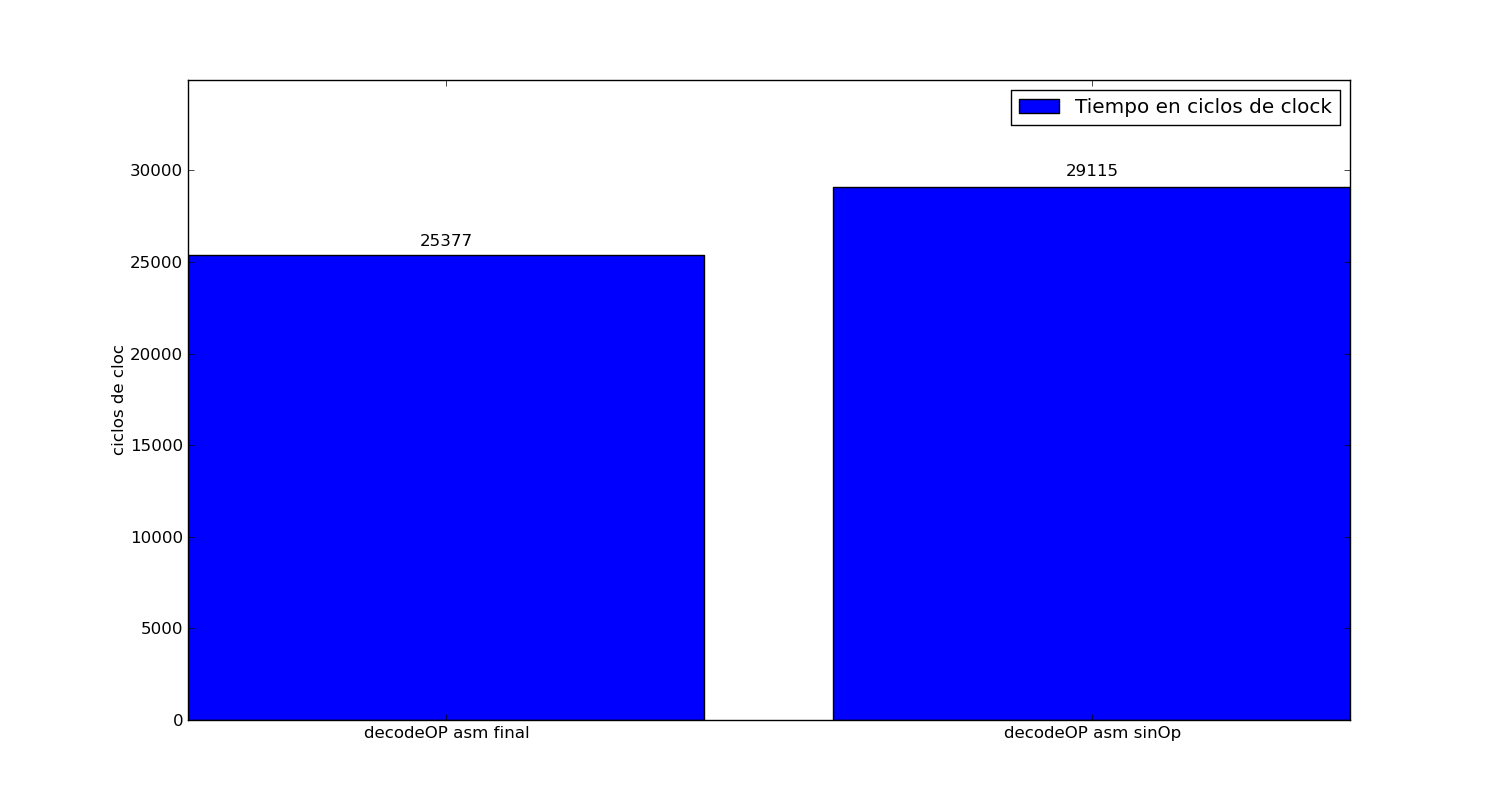
\includegraphics[scale=0.4]{secciones/decodificacion/imagenes/decodeOP.png}
\end{center}
\caption{Diferencia de rendimiento entre asm sin entubado de código y asm con entubado de código en 2 etapas}
\label{fig:entubado de codigo}
\end{figure}



	De esta manera el prefijo es sencillamente leer los datos necesarios para la primera iteracion
del ciclo.


	El sufijo por otro lado no existe. El sufijo hipotético debería ser hacer un procesamiento
a mano de los datos, sin embargo esto primero se subsanó haciendo que haya una lectura de datos de más
adentro del ciclo. Luego el sistema para controlar la multiplicidad de \textit{size} lo arregló
por completo.

	A nivel de lógica esta optimización aplicada de esta forma tan básica realmente resultó
muy sencilla. Bastó con agregar unas pocas líneas de código y modificar otras
tantas para tener el entubado de 2 etapas funcionando y conseguir cerca de un 15\% de aumento
de rendimiento.


\subsection{Implementaciones}


	Para decode se usaron 3 implementaciones: Una escrita en lenguaje C.
Una escrita en lenguaje ensamblador y otra escrita en lenguaje ensamblador
intentando usar la máximo los beneficios de la ténica de software pipelining.

	El algorítmo de C al igual que en los otros filtros es lo mas intuitivo posible.
Basicamente se lee de a un byte de la imagen. Mediante máscaras se filtran los dos bits
menos significativos y los siguientes 2 bits menos significativos.

	Los bits 2 y 3 se comparan en un switch para saber como procesar
a los bits 0 y 1. Una vez que se procesaron los bits 0 y 1 se los guarda se los
mueve a izquierda la cantida de lugares adecuada (0, 2, 4 o 6) según sea el primer
par de bits de ese bytes, el segundo, el tercero o el cuarto. Luego se van acumulando
esos resultados parciales y cuando se tiene un byte entero se lo guarda en el vector
destino.

	Cabe aclarar que a la hora de implementar en ensamblador este filtro provee bastantes
facilidades. Todos los corrimientos que hay que hacer son múltiplos de dos y la cantidad
de datos que hacen falta decodidificar para formar un byte es potencia de 2. Estas
cosas facilitaron mucho el trabajo. Además en ningún momento se necesita saber la
posición de los pixeles ni nada por el estilo, por lo que la matriz fuente se puede
tomar sencillamente como un gran vector. Sin embargo existe una dificulad: La
multiplicidad del parámetro \textit{size}. Nada nos asegura que size tenga una
multiplicidad cómoda, por esto es fundamental tener en cuenta esto para poder
procesar en paralelo sin hacer accesos a memoria ilegales y sin dejar de procesar nada.

	A continuación se exlicará el algoritmo usado para el filtro en asm dejando de lado
el tema de la multiplicidad de size. Este tema se lo va a tratar de manera especial luego.

\subsubsection{Implementación decode ASM: Preparando los datos}

	Las únicas acciones indispensables para poder trabajar con el ciclo son 2: Inicializar
los contadores y traer las máscaras a registros (usarlas desde memoria sería un puñal
en el corazón de la performance). Las máscaras que se utilizan son las siguientes:

\begin{itemize}
	\item Una máscara para filtrar los 2 bits menos significaticos (0x03 repetido 16 veces)
	\item Una máscara para filtrar los bits 2 y 3 (0xC repetido 16 veces)
	\item El número 1 para usar como operando. (0x1 16 veces)
	\item Tres máscaras con los valores que deben tener los bits 2 y 3 en cada una de las posibles operaciones.
	\item Una máscara para filtrar la basura que se acumula durante el recorrido (0x000000FF repetido 4 veces)
	\item Una máscara con las posiciones para el shuffle final (0x00, 0x04, 0x08, 0xC, 0x08 repetido 12 veces).
\end{itemize}

	Luego hay 2 procesos más mas se deben realizar. El primero es traer datos del destino
a un registro xmm. Esto sería el prefijo del entubado de código. Por supuesto
a esto sigue aumentan en 16 el contador del destino.

	Por último hay que hacer una serie de operaciones para tratar la multiplicidad
de size. Sobre eso se hablará después.


\subsubsection{Implementación decode ASM: El ciclo}


	El ciclo sencillo, pues es una adaptación fiel del algoritmo intuitivo
al procesamiento SIMD.
	
	En un comienzo se traen nuevos datos. Sin embargo no se trabaja con esos datos,
se trabaja con los datos que se habían alojado previamente en xmm0. Los nuevos datos
no se los usa hasta el ciclo siguiente.

	El procesamiento en si comienza copiando los datos y aplicando
en cada copia un filtro distinto mediante un AND empaquetado con máscaras.
en una de las copias se dejan sólo los 2 bits menos significativos, en la siguiente
sólo los siguientes dos bits menos significativos (el 2 y el 3). A continuación
se repite el mismo esquema de trabajo para las 3 posibles operaciones
que se deben realizar sobre los datos.

	Se copian el registro que contiene los bits 2 y 3, se usa la copia para crear
una máscara que indica donde se debe aplicar la operación y donde no, se
hace un AND empaquetado entre esa máscara y otra máscara estática que contiene
el operando. Se realiza la operación entre el registro que tiene los bits
0 y 1 y la última máscara creada.

	El siguiente esquema muestra todo esto:

\begin{figure}[h]
\begin{center}
  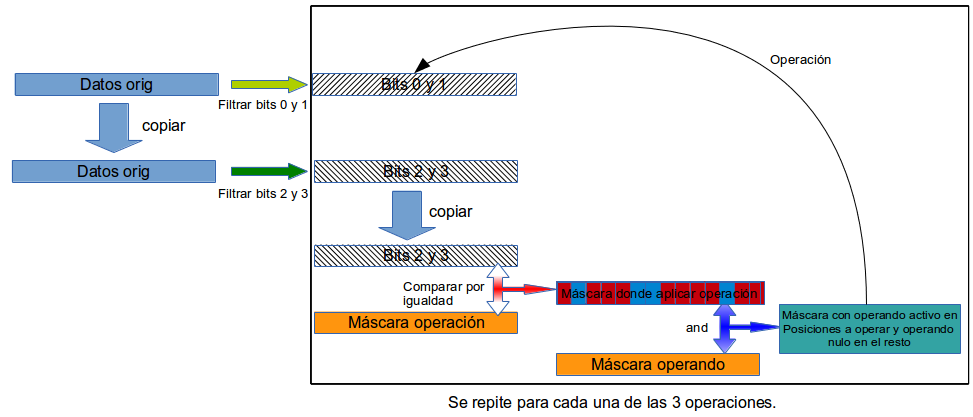
\includegraphics[scale=0.6]{secciones/decodificacion/imagenes/esquemaCicloDecode.png}
\end{center}
\caption{Esquema de funcionamiento de la primera parte del ciclo de decode.}
\label{fig:ciclo-decode}
\end{figure}


	Una vez hecho esto lo único que falta es acomodar los datos y grabarlos.

	Terminado todo esto se hacen avanzar los punteros y se mueven los datos que se
trajeron al registro xmm0 para poder procesarlos en la próxima iteración.

	A esta altura es importante remarcar una cosa que tal vez no se notó tanto.
El entubado de código en dos etapas (que aumentó el rendimiento en cerca del 15\%)
sólo agrega unas pocas líneas de código al ejercicio:


\begin{minted}[linenos,stepnumber=1]{nasm}

	MOVDQA xmm0, [rdi]

;(logica para la multiplicidad de size)

ciclo:

	MOVDQU xmm7, [rdi+r9] ; Se traen datos nuevos  se los guarda en un registro auxiliar

;---------------------------------------------------------------
;--------Cuerpo del ciclo usando los datos de xmm0--------------
;---------------------------------------------------------------

	MOVDQA xmm0, xmm7; Se dejan los datos en xmm0 para poder usarlos la proxima iteracion

;---------------------------------------------------------------
;--------Final del ciclo y logica para multiplicidad de size----
;---------------------------------------------------------------

\end{minted}

	Esas 3 líneas de código son las únicas realmente involucradas con
el entubado de código. Es decir que usar el entubado de código de esta forma
realmente tiene una gigantezca relación costo beneficio.



\newpage

\subsubsection{Implementación decode ASM: La multiplicidad de \textit{size}}

	El problema de la multiplicidad de size es un problema sencillo que
obliga a agregar mas lógica de la que pareciera. El problema en esta implementación
de este filtro es que se usan 2 contadores simultaneos (uno para \textit{src} y otro
para \textit{dst} ) y cada uno avanza a otra velocidad. Sin embargo \textit{size} se
compara con uno sólo de ellos para saber cuando parar de iterar, la consecuencia
de ello es que cuando la multiplicidad de size no es la adecuada hay que modificar
los dos contadores de manera diferente.

	La solución que se le dió a esta problemática en esta implementación está
dividida en 2 etapas: Antes de entrar al ciclo se calcula cuanto va a tener
que retroceder el contador de \textit{src}.

\begin{minted}[tabsize=4]{nasm}

	MOV    r8, rdx  ; Se copia size
	SHL    r8, 62   ; Se conservan los ultimos 2 bits (resto modulo 4)		
	SHR    r8, 62   ; Se vuelve al estado original
	MOV    rcx, 4   ; En otro registro se trae un 4
	SUB    rcx, r8  ; Ahora en rcx esta lo que falta a rdx para ser modulo 4
	SHL    rcx, 2   ; Finalmente se lo multiplica por 4. Esto es lo que queremos que
                    ; retroceda el contador de fuente que avanza 4 veces mas rapido
									
	ADD    rcx, 16  ; Se suma 16 a rcx para compensar que el contador siempre esta
                    ; una iteracion mas adelante que el proceso de datos por el
                    ; entubado de codigo

	XOR	   r8, r8 	; r8 se usa como flag al final del ciclo.						

\end{minted}


	La segunda parte es un sector del ciclo al que sólo se accede en la última
iteración. Basicamente lo que se hace es mover el límite de se hace es
poner al contador de \textit{dst} (r10) en la posición exacta a la que debe
quedar (\textit{size}-4) y hacer retroceder al contador de destino
con la cifra calculada antes. Además se cambia el flag indicando que ya
se pasó por ahí para que efectivamente sea la última iteración.



\begin{minted}[tabsize=4]{nasm}

	JL       ciclo           ; Final del ciclo

	MOV      r10, rdx        ; Se pone el contador de dst en size-4
	SUB      r9, rcx         ; Se hace retroceder el contador de src la cantidad adecuada
	MOVDQU   xmm0, [rdi+r9]  ; Se ponen en xmm0 los datos adecuados para la ultima iteracion
	CMP      r8, 0           ; Se verifica que sea la primera vez que se entra al ciclo.
	MOV      r8, 1           ; Se setea el flag en "ya se visito este lugar"
	JE       ciclo           ; Si el flag estaba en cero se salta a ciclo. 
                                ; (notar que MOV no modifica eflags)

\end{minted}


	Esta solución para este problema tiene como principal problema
que siempre se realiza una iteración de más, por mas que la multiplicidad
de \textit{size} sea la correcta. Sin embargo los ciclos
de este filtro son realmente muy rápidos, por lo que eso no resulta
un problema mayor.

\newpage

\subsection{Rendimiento}

\begin{figure}[h]
\begin{center}
  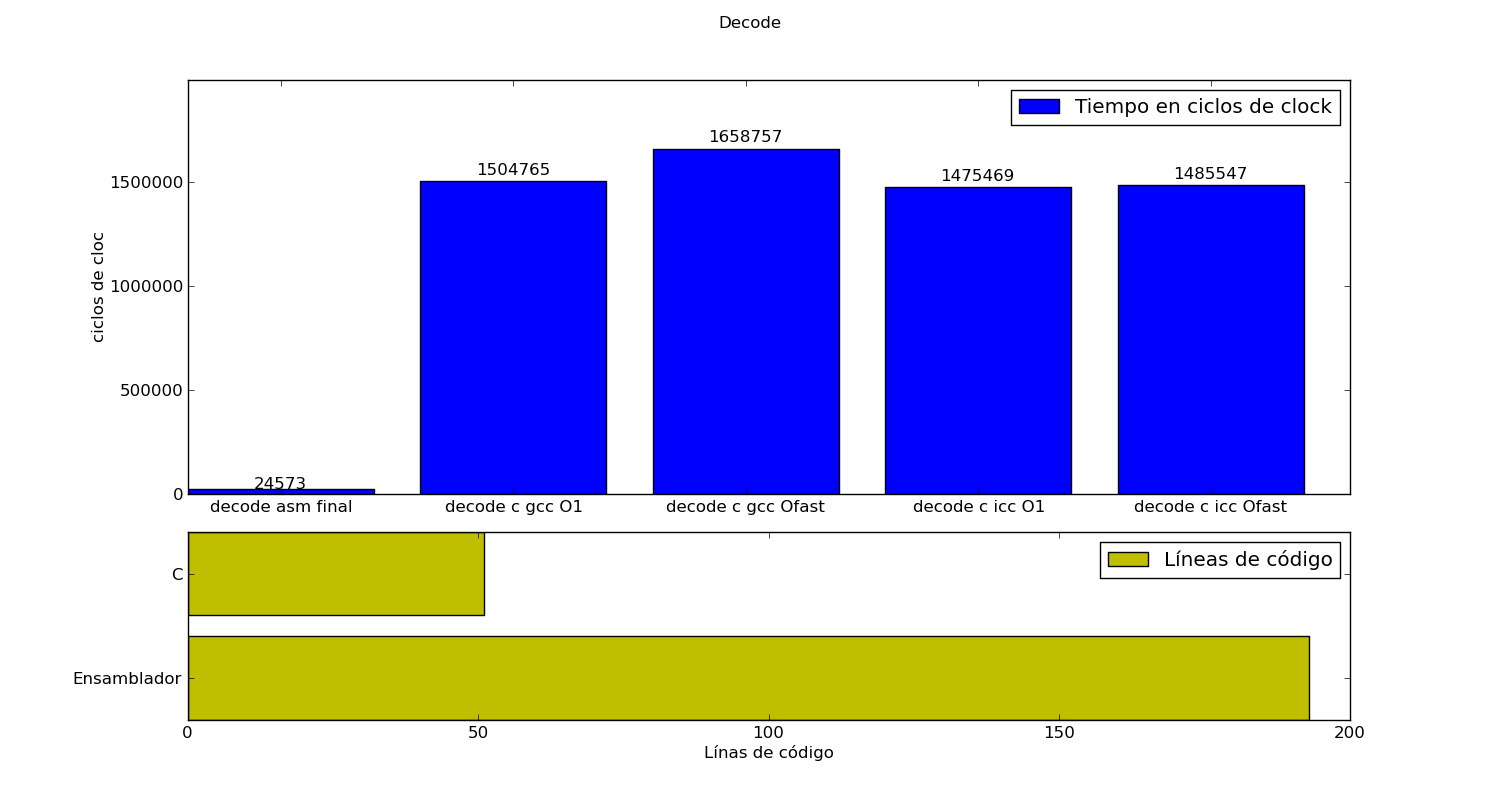
\includegraphics[scale=0.5]{secciones/decodificacion/imagenes/decode.png}
\end{center}
\caption{Rendimiento de las diferentes implementaciones.}
\label{fig:rendimiento decode}
\end{figure}

	Como se puede ver en el gráfico el rendimiento de la versión en assembler es notablemente mas rápida. Otra
vez no cumple con la hipótesis inicial. La versión en ASM es más de 60 veces mas rápida que la versión
de C. Al introducir ICC en la ecuación la cosa cambia un poco, sin embargo el resultado sigue siendo que
la versión en ensamblador aplasta a las demás.

	En este momento cabe volver a mencionar que este filtro calza a la perfección en el procesamiento
SIMD con SSE. Aclarado esto vamos a ahondar un poco más.

	La versión de C siguiendo el código tal cuál está escrito accede a memoria 5 veces cada 4 bytes.
Es decir, tiene que buscar cada byte. Luego de procesar 4 bytes tiene que ir a guardarlos. Es decir
que suponiendo que el compilador genera un código que no accede nunca a memoria durante el ciclo de todas
maneras se están accediendo 20 veces a memoria cada 16 bytes. La versión escita en ensamblador, en cambio
realiza sólo 2 accesos cada 16 bytes (uno para traer datos, otro para guardarlos). Pero no sólo eso sino
que además el acceso mas conflictivo (el de trar datos) está optimizado mediante entubado de código.

	Otra cosa importante a la hora de hacer este análisis es que se sabe con mucha presición
cuantas veces se realiza el ciclo principal. Si o si está en el orden de $size/4$ veces. Es decir,
en cada iteración se graban exactamente 4 bytes y las iteraciones terminan cuando se graban $size$ bytes
por lo tanto ese va a ser el total de iteraciones.

	Despreciando las instrucciones de afuera del ciclo (que tiene sentido porque son pocas y se
realizan una sóla vez) la cantidad de ciclos de clock por iteración entonces va a ser el cociente
entre los clocks totales y $size/4$. Eso da proximamente 9,2. Sin embargo el ciclo tiene 36
instrucciones, lo que quiere decir que se logró aproximadamente un rendimiento de 4 instrucciones
por ciclo de clock.

